\documentclass[tikz,border=8pt]{standalone}
% Shared look for every TikZ diagram. Load with \input{../../tools/tikz-style.tex}
\usepackage[T1]{fontenc}
\usepackage{lmodern}
\renewcommand{\sfdefault}{lmr}  % diagrams use the same serif as the text
\usetikzlibrary{arrows.meta, positioning, shapes.geometric, calc, fit, backgrounds}
\definecolor{cblue}{HTML}{4C78A8}
\definecolor{corange}{HTML}{F58518}
\definecolor{cgreen}{HTML}{54A24B}
\definecolor{cred}{HTML}{E45756}
\definecolor{cpurple}{HTML}{B279A2}
\definecolor{cgrey}{HTML}{6B6B6B}
\tikzset{
  every picture/.style={font=\sffamily, line width=1.2pt},
  box/.style={draw=#1, fill=#1!12, rounded corners=4pt, align=center, inner sep=7pt, minimum height=1.1cm},
  box/.default=cgrey,
  arrow/.style={-{Stealth[length=3mm]}, draw=cgrey, line width=1.4pt},
  title/.style={font=\sffamily\bfseries\Large},
  note/.style={font=\sffamily\small, text=cgrey, align=center},
}
\AtBeginDocument{\hyphenpenalty=10000 \exhyphenpenalty=10000}

\begin{document}
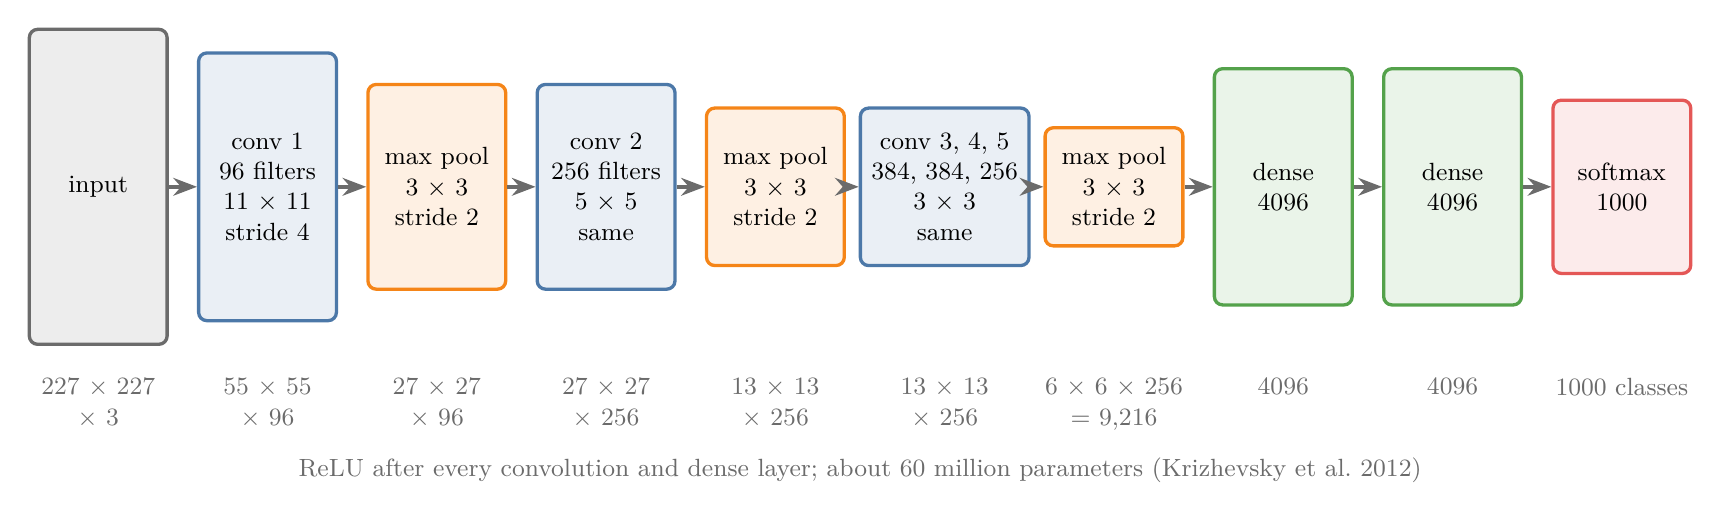
\begin{tikzpicture}[
    layer/.style={draw=#1, fill=#1!12, rounded corners=3pt, align=center, inner sep=4pt,
                  minimum width=1.75cm, font=\sffamily\small},
    dims/.style={font=\sffamily\small, text=cgrey, align=center}]
  % name, colour, height (cm), label under the box
  \foreach \i/\name/\col/\h/\out in {
      0/{input}/cgrey/4.0/{227 $\times$ 227\\$\times$ 3},
      1/{conv 1\\96 filters\\11 $\times$ 11\\stride 4}/cblue/3.4/{55 $\times$ 55\\$\times$ 96},
      2/{max pool\\3 $\times$ 3\\stride 2}/corange/2.6/{27 $\times$ 27\\$\times$ 96},
      3/{conv 2\\256 filters\\5 $\times$ 5\\same}/cblue/2.6/{27 $\times$ 27\\$\times$ 256},
      4/{max pool\\3 $\times$ 3\\stride 2}/corange/2.0/{13 $\times$ 13\\$\times$ 256},
      5/{conv 3, 4, 5\\384, 384, 256\\3 $\times$ 3\\same}/cblue/2.0/{13 $\times$ 13\\$\times$ 256},
      6/{max pool\\3 $\times$ 3\\stride 2}/corange/1.5/{6 $\times$ 6 $\times$ 256\\= 9,216},
      7/{dense\\4096}/cgreen/3.0/{4096},
      8/{dense\\4096}/cgreen/3.0/{4096},
      9/{softmax\\1000}/cred/2.2/{1000 classes}} {
    \node[layer=\col, minimum height=\h cm] (L\i) at (2.15*\i, 0) {\name};
    \node[dims, anchor=north] at (2.15*\i, -2.3) {\out};
  }
  \foreach \i [evaluate=\i as \j using int(\i+1)] in {0,...,8} \draw[arrow] (L\i) -- (L\j);
  \node[note, anchor=north] at (2.15*4.5, -3.3) {ReLU after every convolution and dense layer; about 60 million parameters (Krizhevsky et al.\ 2012)};
\end{tikzpicture}
\end{document}
